% This is the main report file

\documentclass{acm_proc_article-sp}
\usepackage[utf8]{inputenc}
\usepackage{listings}
\begin{document}

\title{02223 Fundamental models for modern embedded systems E10}
\subtitle{[Scheduling deterministic]
\titlenote{This report should also be available online at \texttt{www.retrospekt.dk/02223report}}}

\numberofauthors{1}
\author{
\alignauthor 
Kim Rostgaard Christensen\\
       \email{s084283@student.dtu.dk}
}

\maketitle

\begin{abstract}
%Abstract; A brief summary of all of the report including the conclusion section
%but excluding the acknowledgements, references and any appendixes.
\end{abstract}
% XXX Should this be here? 
% A category with the (minimum) three required fields
%\category{H.4}{Information Systems Applications}{Miscellaneous}
%A category including the fourth, optional field follows...
%\category{D.2.8}{Software Engineering}{Metrics}[complexity measures, performance measures]

%\terms{Report}

%\keywords{ACM proceedings, \LaTeX, text tagging} % NOT required for Proceedings


\section{Introduction}

%Introduction; A discussion putting the work into context and discussing the
%background of the work. The section should include any problem statements
%addressed, a very brief summary of the work carried out, the most import ant
%results and the most important conclusions. The section should end with a
%description of the report structure.



\section{The WCET}
The Worst Case Execution Time is the maximum time a given task can take up the cpu. It has a complimentary cousin called Best Case Execution Time.

%TODO nicer introduction

\subsection{Obtaining WCET}
To be able to obtain the exact WCET it is essential that the all about the hardware architecture is known.
%TODO More on this

Modern processors tend to try and make things run faster by utilizing pipelines, instruction caches and branch prediction.

\subsubsection{Branch prediction}
When a branch in the program is reached (for example an if statement), the processor will try to predict which route the software will take. This saves cpu cycles, when guessed correctly, but costs extra cycles when an incorrect prediction is made, due to the fact that all the instructions that was lined up, now has to be replaced.

\subsubsection{Pipelining}
%TODO

\subsubsection{Instruction cache}
%TODO

\subsubsection{Virtual memory}
%TODO Virtual memory and why it sould not be used in RTOS
A few suppliers of real-time operating systems gives the programmer the option of using virtual memory, giving the benefit of being able to extend the application. QNX for example has this feature.
The majority of suppliers does not implement virtual memory though, so in most cases this is not an issue.


\section{Very Simple Simulator}
\subsection{Rate monotonic scheduling}
Rate monotonic scheduling (RMS) is a preemptive scheduling algorithm used when you have set of strictly periodic tasks with deadlines equal to their periods. A number of other assumptions are also required. All of them are listed here.
\begin{itemize}
\item Single processor
\item Task deadlines are equal to their periods
\item Periodic tasks
\item All tasks are released as soon as they arrive
\item All tasks start at the same time
\item All tasks are independent
\item No precedence or resource constraints
\item No task can suspend itself
\item All overheads in the kernel are assumed to be zero
\end{itemize}

\subsection{Schedulability}
To determine schedulability of a task set, a utilization test is applied. The formal version of the test is as follows:

\begin{equation}
\displaystyle\sum\limits_{i=1}^{n} \frac{C_i}{T_i} \leq n \left( 2^{\frac{1}{n}} - 1 \right) 
\end{equation}
Or, in other words: The cpu usage represented on the left hand side by the sum of all the individual tasks utilization of the cpu in their period must be less that $n \left( 2^{\frac{1}{n}} - 1 \right) $, where $n$ is the number of tasks.\\
This is a sufficient test, and task sets that fail this test are not necessarily unschedulable.\\\\
Futhermore, it holds that:
\begin{equation}
\underset{y\rightarrow0}{\lim}U_{lub}(n)=\ln2
\end{equation}
Proven by Liu and Leyland.

\subsection{Simulation}
%REMEBER! THIS IS A SIMULATOR - Simulate the running of an embedded application on a single processor system using preemtive fixed-priority scheduling.
For simulating a task set under rate monotonic scheduling, we first have to find a LCM of all the periods for the tasks in the set. This is also known as the hyperperiod. As $C_i$ needs to be randomized, the simulation should run for a number multiples of the hyperperiod. The multiple of LCM will be denoted $n$
\subsubsection*{Priority assignment}
The priorities is in RMS defined as the inverse of the period. In this implementation, the priority is relative to the hyperperiod and defined as $P_i = \frac{LCM}{T_i}$. This is done to avoid rounding errors and floating point arithmetic in simulation.
\subsubsection*{Job initialization}
To initialize the jobs we insert them into a job queue with release time equal to $\tau_{i}.period \cdot (j - 1)$ where $\tau_i$ is the task of the job, and $j$ is j'th occurrence of the task. The job's time  (remaining execution time) is also randomized in this step.
\subsubsection*{Simulation}
The jobs are sorted on start time and priority, and the simulation runs by going through each cycle from 1 to $n$. In each cycle, a list of ready jobs are generated and the job with the highest priority is picked to execute. Ready jobs are jobs that have time > 0 and release < current cycle.\\
Execution is done by a tick method call to the job that decreases time.\\
When the job terminates (time = 0), the response time is recorded and compared to the overall worst-case response time of the task, recording if it is worse that any previous.

\subsection{Output}
The simulator produces a textual output in the form:(name) (WCRT) newline. An example is shown below:
\begin{verbatim}
T1 1
T2 54
T3 2
T4 4
T5 6
T6 10
T7 28
\end{verbatim}
It also returns the schedulability determined by asserting $D_i > WCRT_i$ for each task:
\begin{verbatim}
Simulator.RateMonotonicSimulation Reports Schedulable
\end{verbatim}
In addition the simulator also produces a graphical output in the form of a timeline in svg format. An example is shown i figure \ref{fig:example_timeline_output}

\begin{figure}[h]
\centering
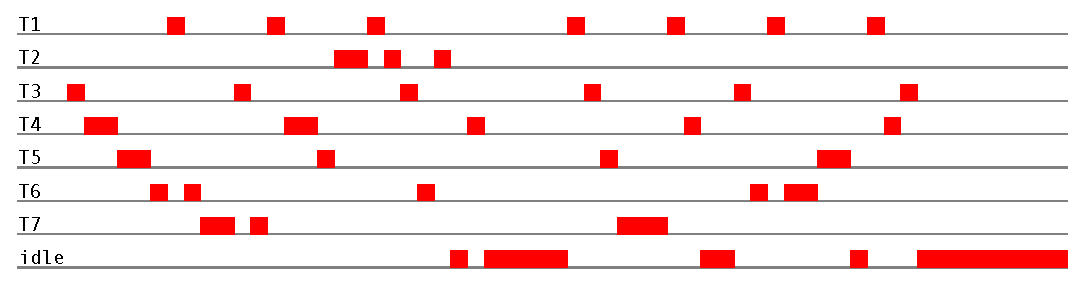
\epsfig{file=fig/example_timeline.eps, height=0.8in}
\caption{Example timeline}
\label{fig:example_timeline_output}
\end{figure}

\subsection{Implementation details}
\subsubsection{Generation of the random numbers}
In order to perform a simulation having both a BCET and WCET, a randomization is needed. For this simulators purpose, either uniform or Gaussian distribution is used, depending on the configuration parameters. On an implementation note, Java's is used java.util.Random class is used for generating the random numbers. When using the uniform distribution the following should be taken into account:

\begin{quotation}
... Returns a pseudorandom, uniformly distributed int value between 0 (inclusive) and the specified value (exclusive) ... All n possible int values are produced with (approximately) equal probability\cite{javadoc16}
\end{quotation}
%TODO set qoute origin

As the upper value is exclusive, we need a value in the range $[BCET:WCET+1[$ when using a uniform distribution.\\
Future improvement could also include to possibility to use a seed, to be able to recreate the random numbers generated.

\subsubsection{Traceability}
To be able to determine the situation of the first time overflow, a timeline is maintained, raising a global flag when the overflow occurs, and record the cycle.\\
%Can you determine what situation created the worst-case response time for a particular task (what other tasks interrupted it, when, and for how long)?
To be able to trace what other task interrupted it, we can go back to the point where the overflown task last stopped (in time) and record the tasks between them.

\subsubsection{Response time guarantee}
%Can you guarantee that the response time will not be larger than the worst-case numbers you get from the simulator?
When using random execution times are used for simulation, no guarantee can be provided. Although if you have a random distribution that is similar to the one in the actual application, then you are able give a better estimate.\\

% What happens if you simulate using the execution time equal to WCET?
When the execution time is always set to WCET, You end up with a very pessimistic estimate on the response time - although guaranteed to be accurate. In praxis, a lot of CPU time will be wasted, especially if the execution time is much larger than the typical execution and only happens in very rare or perhaps even in theoretical cases.\\
Effectively you get the same figures as the response time analysis explained in section \ref{sec:rta}.
\subsection{Final thoughts}
Although one of the assumptions is that tasks must be independent, it is not guaranteed that task are statistically independent - meaning that a higher execution time on one task can be due to an external effect, that affects other tasks as well.\\
This eventually leads to a cascade of higher response times on all tasks that depend on, for example, some external input. Due to, that in the real world variables are not always independent.


\section{Response-Time Analysis}
Response-time analysis, in this case, involves the Deadline Monotonic feasibility test. It is based around the assumption that you know you critical instant (see section \ref{sec:critical_instant}) and from this point determines the worst-case response time of each task. Deadline monotonic is optimal for fixed task priority, and falls under the same assumptions as rate monotonic scheduling, with the one exception that deadlines can be less than the period.

\subsection{Analysis}
The analysis is based around the calculation of worst-case interference of a task. Interference of a task is defined as this:
\begin{equation}
I_{i}= \displaystyle\sum\limits_{j=1}^{i-1} \left\lceil \frac{R_{i}^{k}}{T_{j}}\right\rceil C_{j}
\end{equation}
Meaning that the worst-case interference a task can experience is the response time of all previous tasks. Hence the total response time of the task becomes:
\begin{equation}
R_{i}=C_{i} + \displaystyle\sum\limits_{j=1}^{i-1} \left\lceil \frac{R_{i}^{k}}{T_{j}}\right\rceil C_{j}
\end{equation}
I order to calculate this, we need to iterate through all the tasks with higher priority than the one we are currently examining, add up all the response times to the current task and record previously calculated response times.\\
Only the task with the lowest priority needs to be analysed in order to guarantee schedulability.
\subsection{Implementation details}
This response time analysis (deadline monotonic) is extended from an abstract analysis class, that has some properties general for all analysis's. This enables modularity and extensibility.\\
The implementation gives roughly the same textual output as the Very Simple Simulator, obviously without the svg timeline.
\subsubsection{Comparison of RTA response times}
%How do the worst-case response times you get with RTA compare to those you get with VSS?
The worst case response times are the same as the ones in the Very Simple Simulator when $T_i = D_i$.
This is due to the fact, that the algorithms are very similar in effect. This hold specifically when $C_i=WCET_i $.

%How many simulation runs do you need to run VSS to get the same numbers? 
\subsubsection{Comparison with Very Simple Simulator}
In order to get the same numbers as with the VSS, you would need to run the simulation once with $C_i=WCET_i$, or infinite with random values, due to:
\begin{equation}
\underset{n\rightarrow \infty }{\lim}C_i=WCET_i\end{equation}
%Can you modify the algorithm to determine what situation created the worst-case response time for a particular task? - no



\section{Something advanced}
%\subsection{Rate monotonic scheduling}
Rate monotonic scheduling (RMS) is a preemptive scheduling algorithm used when you have set of strictly periodic tasks with deadlines equal to their periods. A number of other assumptions are also required. All of them are listed here.
\begin{itemize}
\item Single processor
\item Task deadlines are equal to their periods
\item Periodic tasks
\item All tasks are released as soon as they arrive
\item All tasks start at the same time
\item All tasks are independent
\item No precedence or resource constraints
\item No task can suspend itself
\item All overheads in the kernel are assumed to be zero
\end{itemize}

\subsection{Schedulability}
To determine schedulability of a task set, a utilization test is applied. The formal version of the test is as follows:

\begin{equation}
\displaystyle\sum\limits_{i=1}^{n} \frac{C_i}{T_i} \leq n \left( 2^{\frac{1}{n}} - 1 \right) 
\end{equation}
Or, in other words: The cpu usage represented on the left hand side by the sum of all the individual tasks utilization of the cpu in their period must be less that $n \left( 2^{\frac{1}{n}} - 1 \right) $, where $n$ is the number of tasks.\\
This is a sufficient test, and task sets that fail this test are not necessarily unschedulable.\\\\
Futhermore, it holds that:
\begin{equation}
\underset{y\rightarrow0}{\lim}U_{lub}(n)=\ln2
\end{equation}
Proven by Liu and Leyland.

\subsection{Simulation}
%REMEBER! THIS IS A SIMULATOR - Simulate the running of an embedded application on a single processor system using preemtive fixed-priority scheduling.
For simulating a task set under rate monotonic scheduling, we first have to find a LCM of all the periods for the tasks in the set. This is also known as the hyperperiod. As $C_i$ needs to be randomized, the simulation should run for a number multiples of the hyperperiod. The multiple of LCM will be denoted $n$
\subsubsection*{Priority assignment}
The priorities is in RMS defined as the inverse of the period. In this implementation, the priority is relative to the hyperperiod and defined as $P_i = \frac{LCM}{T_i}$. This is done to avoid rounding errors and floating point arithmetic in simulation.
\subsubsection*{Job initialization}
To initialize the jobs we insert them into a job queue with release time equal to $\tau_{i}.period \cdot (j - 1)$ where $\tau_i$ is the task of the job, and $j$ is j'th occurrence of the task. The job's time  (remaining execution time) is also randomized in this step.
\subsubsection*{Simulation}
The jobs are sorted on start time and priority, and the simulation runs by going through each cycle from 1 to $n$. In each cycle, a list of ready jobs are generated and the job with the highest priority is picked to execute. Ready jobs are jobs that have time > 0 and release < current cycle.\\
Execution is done by a tick method call to the job that decreases time.\\
When the job terminates (time = 0), the response time is recorded and compared to the overall worst-case response time of the task, recording if it is worse that any previous.

\subsection{Output}
The simulator produces a textual output in the form:(name) (WCRT) newline. An example is shown below:
\begin{verbatim}
T1 1
T2 54
T3 2
T4 4
T5 6
T6 10
T7 28
\end{verbatim}
It also returns the schedulability determined by asserting $D_i > WCRT_i$ for each task:
\begin{verbatim}
Simulator.RateMonotonicSimulation Reports Schedulable
\end{verbatim}
In addition the simulator also produces a graphical output in the form of a timeline in svg format. An example is shown i figure \ref{fig:example_timeline_output}

\begin{figure}[h]
\centering
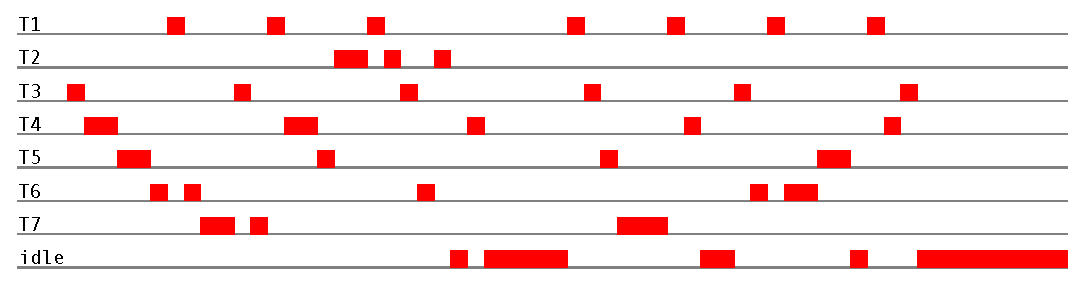
\epsfig{file=fig/example_timeline.eps, height=0.8in}
\caption{Example timeline}
\label{fig:example_timeline_output}
\end{figure}

\subsection{Implementation details}
\subsubsection{Generation of the random numbers}
In order to perform a simulation having both a BCET and WCET, a randomization is needed. For this simulators purpose, either uniform or Gaussian distribution is used, depending on the configuration parameters. On an implementation note, Java's is used java.util.Random class is used for generating the random numbers. When using the uniform distribution the following should be taken into account:

\begin{quotation}
... Returns a pseudorandom, uniformly distributed int value between 0 (inclusive) and the specified value (exclusive) ... All n possible int values are produced with (approximately) equal probability\cite{javadoc16}
\end{quotation}
%TODO set qoute origin

As the upper value is exclusive, we need a value in the range $[BCET:WCET+1[$ when using a uniform distribution.\\
Future improvement could also include to possibility to use a seed, to be able to recreate the random numbers generated.

\subsubsection{Traceability}
To be able to determine the situation of the first time overflow, a timeline is maintained, raising a global flag when the overflow occurs, and record the cycle.\\
%Can you determine what situation created the worst-case response time for a particular task (what other tasks interrupted it, when, and for how long)?
To be able to trace what other task interrupted it, we can go back to the point where the overflown task last stopped (in time) and record the tasks between them.

\subsubsection{Response time guarantee}
%Can you guarantee that the response time will not be larger than the worst-case numbers you get from the simulator?
When using random execution times are used for simulation, no guarantee can be provided. Although if you have a random distribution that is similar to the one in the actual application, then you are able give a better estimate.\\

% What happens if you simulate using the execution time equal to WCET?
When the execution time is always set to WCET, You end up with a very pessimistic estimate on the response time - although guaranteed to be accurate. In praxis, a lot of CPU time will be wasted, especially if the execution time is much larger than the typical execution and only happens in very rare or perhaps even in theoretical cases.\\
Effectively you get the same figures as the response time analysis explained in section \ref{sec:rta}.
\subsection{Final thoughts}
Although one of the assumptions is that tasks must be independent, it is not guaranteed that task are statistically independent - meaning that a higher execution time on one task can be due to an external effect, that affects other tasks as well.\\
This eventually leads to a cascade of higher response times on all tasks that depend on, for example, some external input. Due to, that in the real world variables are not always independent.


%Body; A number of sections describing the work done.

\section{Conclusion}
\label{sec:conclusion}
%Conclusions; All experiences and conclusions drawn from the work.
%The group widely known as group 42 would like to thank everyone for their support and free coffee.\\

\subsection{Threading}
The threading works rather well, but is very limited as it only has one thread in a process. If this was to be implemented, most of the
process handling code should be rewritten.

\subsection{Scheduling}
% ready for multithreading in processes.


%ACKNOWLEDGMENTS are optional
%\section{Acknowledgments}
%\input{acknowledgements.tex}
%Acknowledgments; Acknowledge any persons important to the work.

%References; A list of reference material used. All material must be cited in the
%text.


\appendix


% The following two commands are all you need in the
% initial runs of your .tex file to
% produce the bibliography for the citations in your paper.
\bibliographystyle{plain}
\nocite{*}
\bibliography{sigproc}  % sigproc.bib is the name of the Bibliography in this case
% You must have a proper ".bib" file
%  and remember to run:
% latex bibtex latex latex
% to resolve all references
%
% ACM needs 'a single self-contained file'!
%
%APPENDICES are optional


%Appendixes; Appendixes holds, for example, results or figures that are not
%relevant to place in the body of the report. Appendixes should generally be
%avoided and might not be read by the course staff.


\end{document}
